\chapter{}
``You're mad, aren't you?'' Monique asked. We were on our way back home, and I hadn't said
much. I was a bit pissed at her. Weeks in a hip spica can have bad outcomes. Being with her in
that cast would be enjoyable, but my worry for her safety was overriding that.

\begin{thought}
Monique was worried. Since they'd left the mall, Quinn had been very quiet. He'd not been
receptive to her ideas about long term casts before, and now that the chance meeting had forced
them into a situation that would make a term cast the best escape, she was worried that she'd
really upset him.
\end{thought}

``A little bit. Mostly, I'm worried,'' I answered. ``I've told you before that I don't like
the idea of you wearing a term cast, but the reason I don't like it is because of the risks.
Being with you in that big cast is great. I really love it. I love taking care of you, too- I
really do.''

``Then what's the problem?''

``Well, for one, you're guaranteed to be stiff as hell when it comes off. And if you're
lucky, that's the only problem you'll have. If we're not so lucky, you can lose muscle mass in
your legs from non- use. There can be pressure sores and other skin problems. But, what scares
me the most are the possible circulatory problems- you could develop a blood clot that could
break loose and go to your brain and cause a stroke, or go to your heart or a lung and kill you
instantly.''

\begin{thought}
Monique knew about these things. She'd read about them on the internet. She'd secretly
wanted for several weeks to do a term cast, but knew Quinn would never agree to it for these
reasons. She hadn't planned to wear this one for more than the weekend, and in her desire for a
term cast hadn't really envisioned doing it in a cast this big. But, when Angie and Kaye had
bumped into them at the mall, she'd dropped into the cover story she'd been using all day
without even thinking of the ramifications initially.

When it occurred to her that the story required her to be in the cast for a while, the idea
of wearing it longer quickly became VERY appealing to her, though. She just had to convince
Quinn.
\end{thought}

``Quinn, I know about those risks. And you don't know how much I love it that you're
concerned about me. I swear that I didn't plan this. When Angie and Kaye asked about my cast, I
just started into the story without thinking about the implications.'' She said.

``Monique, I love you. There's so much about you that I never expected to find in a woman.
And I love it that you've taken to recreational casting so enthusiastically. I know you've
wanted to do a term cast, but that one is just too risky. I can't have this hurting you or
worse.''

``Let's just get home. We'll figure out what to do once we get there.'' Monique said.

Once we were home, I unloaded Monique and took her inside. She asked me to plug in her
laptop for her while I unloaded everything. While I brought in everything else, she was busily
tapping away at the keyboard. When I had everything unloaded and put away, I joined her.

``Okay, I did a bit of research,'' she started. ``I have a plan. Hear me out on this, because
it will not only work, we could have some fun with it.''

``Alright,'' I said tentatively.

``First, let's remember exactly what I said to them at the mall: I told them that I got hurt
in the tornado. That was at the end of May. That was three months ago. If I had really been
wearing a cast that long, I would be well on my way to being healed.''

``As long as the injuries weren't too severe,'' I added.

``True,'' she went on. ``But, if I remember correctly, I never even told them exactly what
sort of injuries I have.''

``Not quite. You told them something about getting two leg casts once your hip and pelvis
healed.''

``Ahh, that's right,'' she said. She thought a minute. ``But it still works. So, let's say my
injuries were a broken leg and ankle on the right, a broken leg on the left, and non displaced
breaks to the left hip and pelvis. The doctors wanted to do surgery, but I wouldn't allow it out
of fear of anesthesia, vanity over scarring, or both.''

``Monique, the story doesn't bother me- the risks to your health do!''

``Just wait. Please hear me out. I think I know how we can minimize the risks, and avoid the
embarrassment of showing up tomorrow without a cast. And have a bit more fun with this adventure
while we're at it.''

I let Monique lay out her idea without interrupting her. Her idea was to continue wearing
the plaster hip spica she was in through her first week of school. During that time, she would
mention a few times how difficult it was, lying almost flat and trying to do her school work.
Next Friday, we would cut her out of the cast, and she would spend the weekend hidden in the
house and exercising a lot. Sunday night, we would put her in a new double hip spica. She would
claim that the doctor had said she wasn't ready to be out of the big cast, but he changed it for
one in a seated position so school would be easier. The following weekend, we would again cut
her out for the weekend, and again, recast her on Sunday night, and she would pass it off as the
same cast. These seated hip spicas would be done in fiber for quicker drying.

After the 3rd week of school, we'd take her out of the DHS and put her in individual leg
casts, and she'd continue with those for a month before being out for good. In addition to
spending each weekend cast free, she would do as much exercise as possible during the week for
circulation, and she would drink green tea and take ginseng supplements to reduce the
possibility of forming clots. She said that she'd found that deep vein thrombosis was a minimal
risk for someone her age in good health, and she backed it up with research.

She'd made a good case for it. She really wanted to do it. And, to be completely honest, so
did I. With the health risks minimized, I agreed to be her partner in crime.

She held out her arms for an embrace, and I went to her and held her.

``Thank you.'' She said softly, and then added ``You know, this cast really makes me feel
sexy. And there's only one person on earth I'd want to celebrate that with. Take me upstairs?''

Monday morning, we got up early. I gave Monique a sponge bath, helped her dress, and then
propped her in front of the vanity so she could do her hair and makeup. When she was done, I
loaded her into the wheelchair and we headed for her SUV. Loading her in wasn't getting any
easier, but I'd had an idea for this. The sudden change in the situation necessitated speeding
that project along. She had a class in the morning, and one in the afternoon. While she was in
her morning class, I was going to go to a local shop and set things into motion.

When I moved her from the truck to the wheelchair, we got glances from a few people in the
parking lot. As we moved into the building, we encountered more people, and almost every one of
them, male and female, took a look at the wheelchair-bound Monique. Most of them quickly turned
back to hurrying to their classes, but a few seemed to watch a bit.

It wasn't long before we encountered someone she knew. It was a woman in her early thirties
who had shared some classes with Monique in the past. She seemed to be taken aback by the cast
quite a bit, and was very interested in hearing the story, which Monique told as though she'd
told it many times. We couldn't chat too long, as we had to get her to class.

Once in the classroom, a small crowd gathered around her to ask her questions before the
professor arrived and got things started. I made sure that her backpack with her books, laptop
and other supplies was within reach, and excused myself to go run my errand.

When I arrived at the body shop, I talked with the shop manager about the modification I
needed made to the Expedition. We worked through a few different ideas together until we came
upon a solution that we both thought would work. He quoted me a price, and I told him that I was
on a very tight schedule for needing it, and would pay a premium price if the work could be done
tomorrow. He agreed, and I wrote him a check for half of the agreed price so that he could start
gathering the materials and doing preliminary work today. I would bring the truck to him early
tomorrow, and he would do the installation. He took measurements and made notes before I left.

On my way back to get Monique, I stopped and picked us up some lunch. I retrieved her from
her class, and we went outside to the courtyard to eat. She got the usual double takes and
stares from passersby, and we once again were greeted by people she knew. One in particular
seemed to ask questions that were a bit more specific. The questions made me a bit uneasy, but
Monique handled them with ease. She'd truly gotten into the feel of playing an actual victim.
When that student left, Monique looked at me and silently mouthed the words ``Nursing student.''

The afternoon class went pretty much the same as the morning one. She got a lot of
attention and questions before class. I sat with her through this one, and helped her get
whatever she needed from her backpack, as well as helping her with a bathroom break.

\begin{thought}
The day had been a blast for Monique. She enjoyed school anyway, but fielding all of the
questions and getting so much attention had been amazing. Even when Megan, the nursing student,
had been asking the questions from a medical background, she'd enjoyed answering them. She was
confident that she'd played the victim quite well, showing only as much knowledge as someone
who'd found themselves in such a bad predicament would know.

And though it all, there had been the cast. Her legs and hips held immobile by its embrace.
Soft and comfortable on the inside, yet rigid and unyielding. And Quinn. Her love, her friend,
and now her partner in crime. She couldn't wait to get him home.
\end{thought}

Once we were home, I took Monique inside, and we discussed the day. We went over what had
been difficult, hat had been easy, and how we could deal with things better over the next few
weeks. Thankfully, Monique did not have any classes she had to attend on Tuesday, because we
both had some things that we needed to attend to: I needed to drop off the truck at the body
shop for its modifications, and we had to do some clothes shopping for Monique. She'd prepared a
skirt and some underwear to accommodate the cast, but she'd done it planning for a weekend in
the cast, not three weeks. We had to do some shopping early, so that she'd have time to do any
modifications needed. For now, she wanted to do some reading for school. Since she'd been on her
back all day, I wanted to get her on her stomach for a while to change where the pressure on her
skin was. I took her into the room with the hospital bed, and lifted her to the bed, then rolled
her onto her stomach. I left her to her reading while I prepared dinner. After we ate, I excused
myself to clean up.

\begin{thought}
Monique was feeling great about the day. Everything had been great, start to finish. Even
the challenges of eating while lying on her stomach had been fun. There was just one thing left
to make it perfect. She reached down and unclipped her skirt and untying her underwear. She
yanked the clothing from underneath herself. She then pulled off her top and bra. When Quinn
came back, she was wearing nothing but her cast and her best seductive smile. The cast prevented
them from normal lovemaking, but they'd found ways to pleasure one another around the
restrictions over the past few days, and they were getting better and better at it.
\end{thought}

Afterward, we lie together, going over our exact plans for the next day. As we did this, I
rolled her back on to her stomach and drew a sketch of her as we talked. When I'd walked into
the room after doing the dishes, her pose and expression had been so perfect that there was only
one thing I'd wanted more than to draw her. Now that we'd done that other thing, I put her back
into that position and drew her while we planned.

\begin{center}
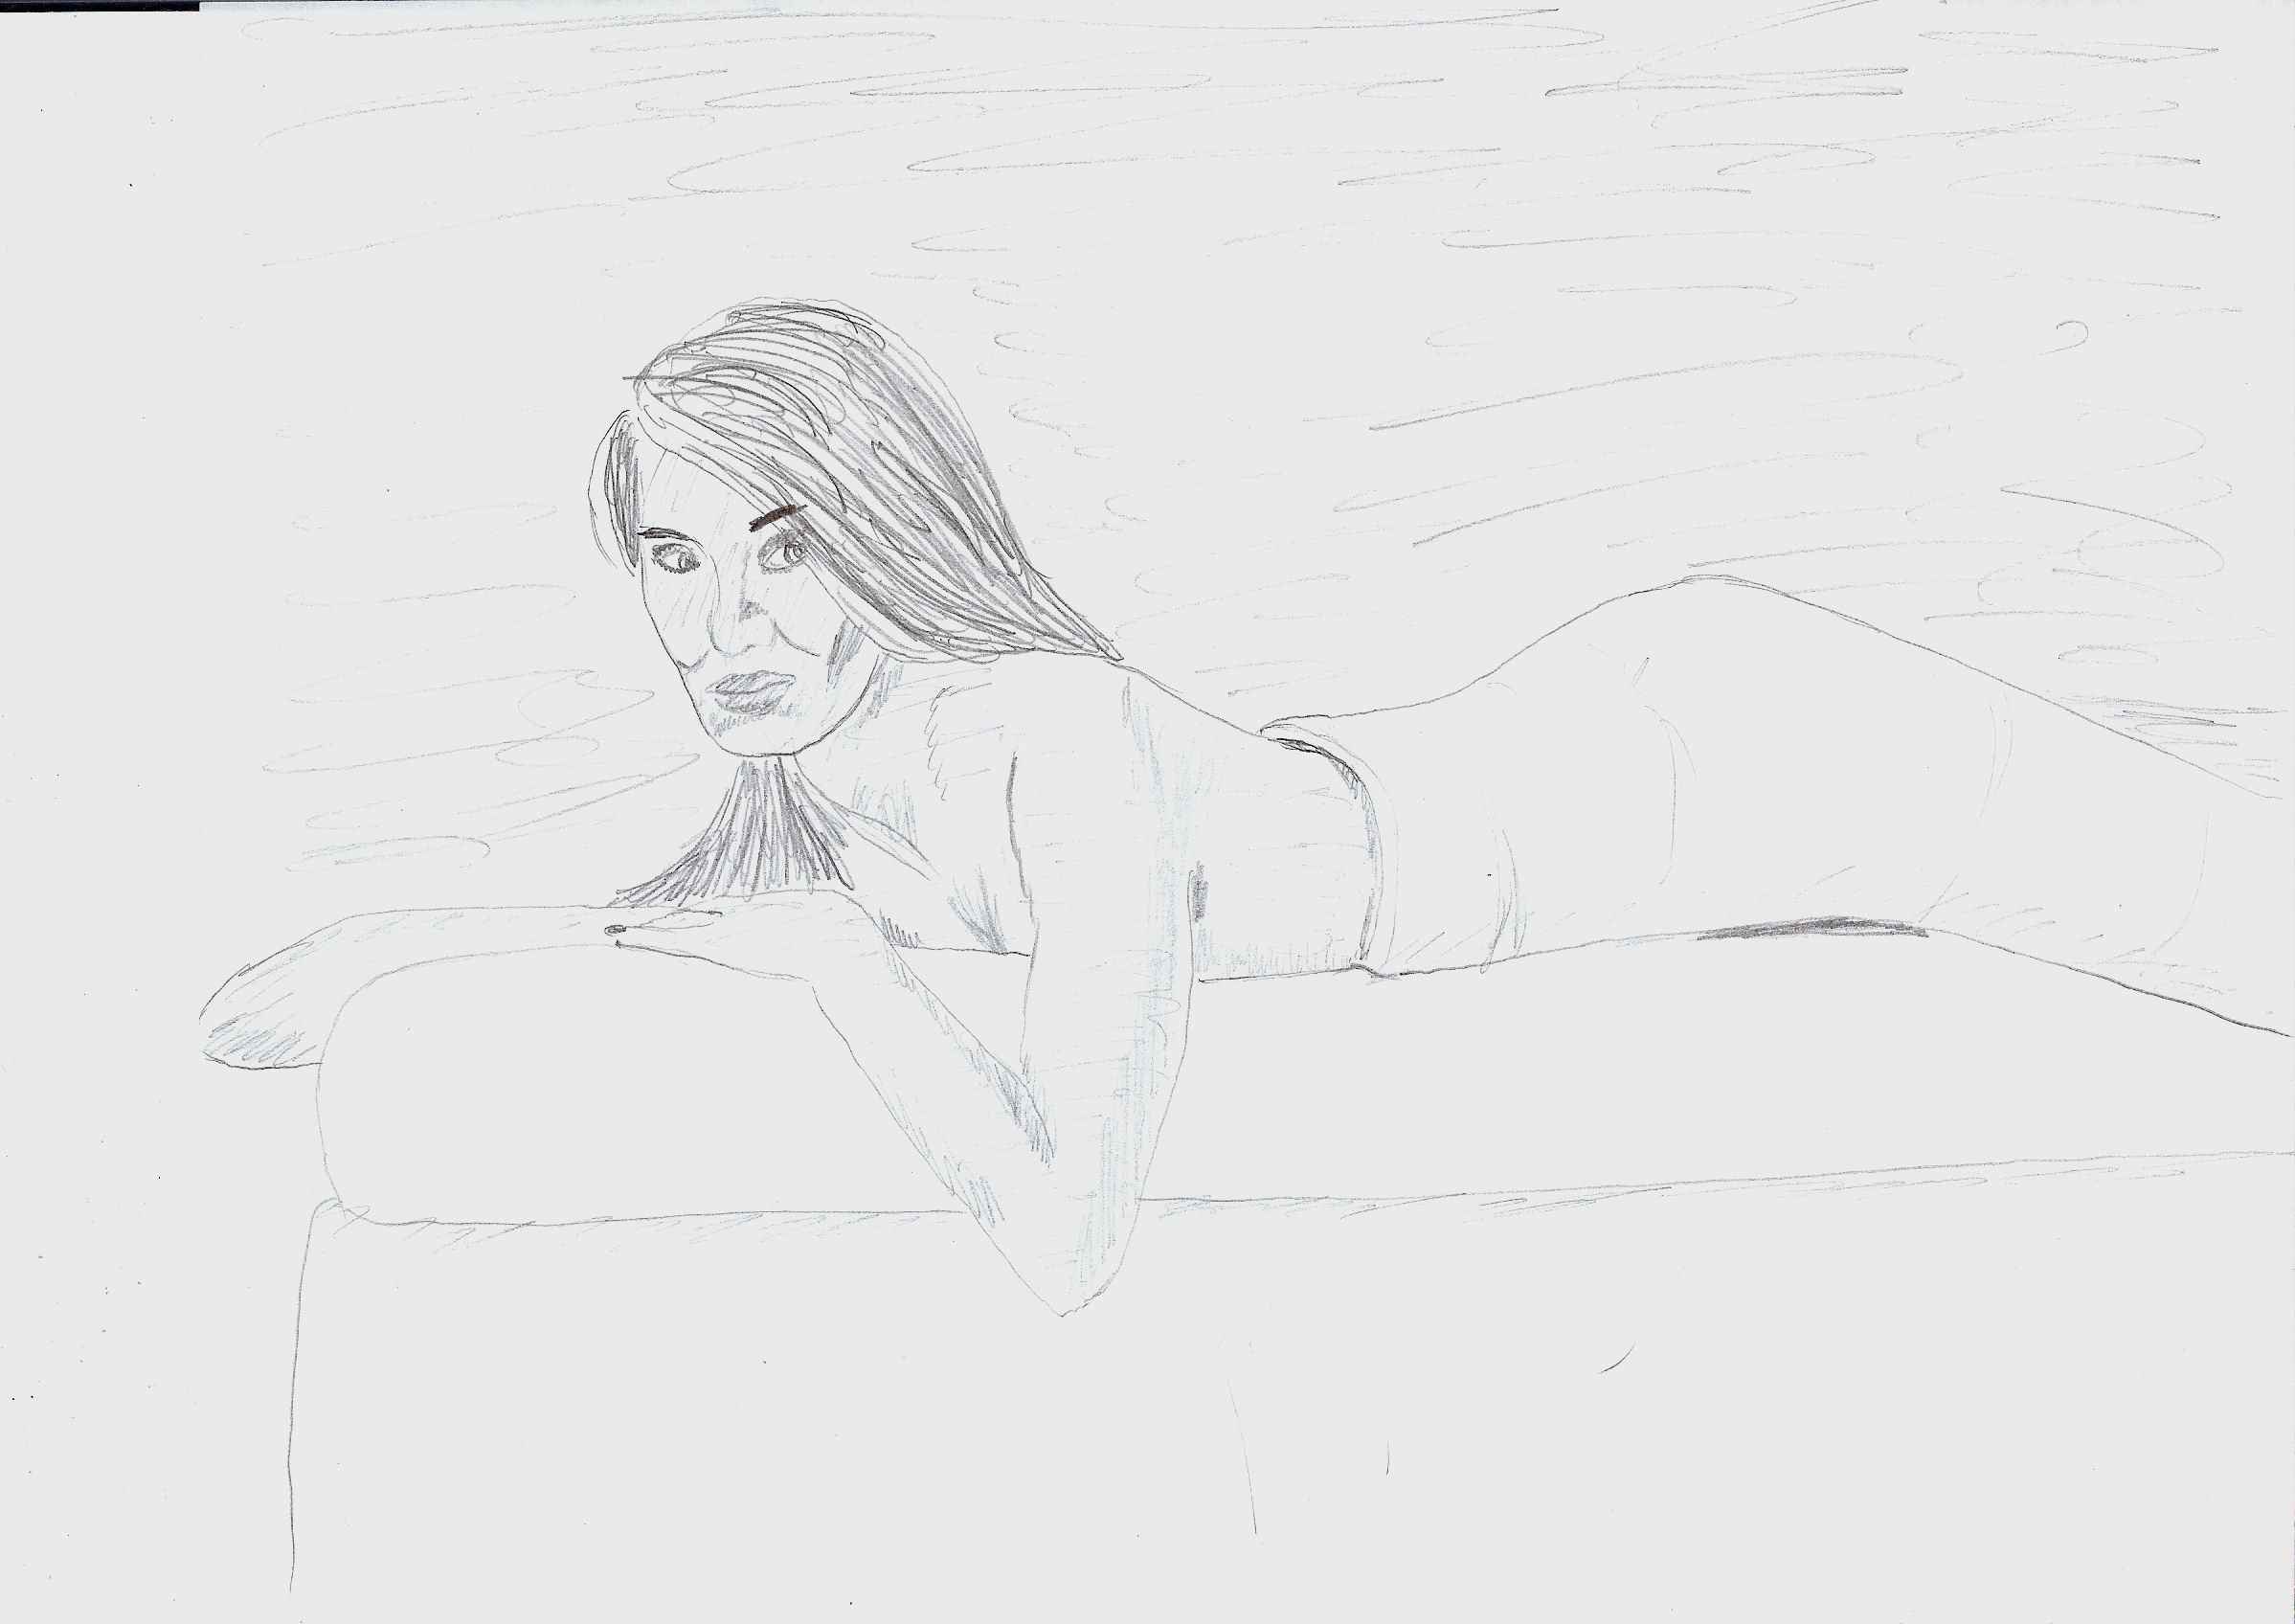
\includegraphics[width=\textwidth]{images/kicks45.jpg}
\end{center}
